\documentclass[a5paper, 10pt]{article}


\usepackage{cite, amsmath, amssymb, booktabs, lastpage, graphicx, float}
\usepackage[hidelinks]{hyperref}

\usepackage{geometry}
\geometry{margin=1.5cm,a5paper,twoside,inner=2cm}

\usepackage{setspace}


\usepackage{amsthm}

\theoremstyle{plain}
\newtheorem{lemma}{Lemma}
\newtheorem{theorem}{Theorem}
\newtheorem{conjecture}{Conjecture}
\newtheorem{proposition}[theorem]{Proposition}
\newtheorem*{corollary}{Corollary}
\renewcommand{\qedsymbol}{\rule{.7em}{.7em}}

\theoremstyle{remark}
\newtheorem*{remark}{Remark}
\newtheorem*{note}{Note}
\newtheorem{case}{Case}

\theoremstyle{definition}
\newtheorem{definition}{Definition}
\newtheorem{example}{Example}

%% Changing the title, author, etc.
\usepackage{graphicx}
\makeatletter
\renewcommand{\maketitle}{
    \begin{center}
    \rule[.2em]{\textwidth}{0.353mm}
        \begin{minipage}[m]{0.35\textwidth}
            {\scriptsize
                \begin{center}
                    \textsf{\textbf{\huge MATCH}\\
                        \textit{Communications in Mathematical\\
                            and in Computer Chemistry}
                    }
            \end{center}}
        \end{minipage}\hfill
        \begin{minipage}[m]{0.65\textwidth}
            \begin{flushright}
                \baselineskip=10px
                {\scriptsize\sffamily{\itshape  MATCH Commun. Math. Comput. Chem.}
                \textbf{\vol{}}
                (\pubyear)
                    \thepage--\pageref{LastPage}}\\
                {\scriptsize\sffamily {\bfseries ISSN:} 0340--6253}\\
                {\scriptsize\sffamily \textbf{doi:} \doi{10.46793/match.\vol-\num.\id}}
            \end{flushright}
        \end{minipage}
        \rule[1em]{\textwidth}{.353mm}
        \baselineskip=0.30in
        {\Large\bfseries \@title} \par
        \vspace{5mm}
        \baselineskip=0.2in
        {\large\bfseries \@author}\par
        \vspace{1mm}
        {\it \@address} \par
        {\small\tt \@email} \par
        \vspace{3mm}
        {\small (Received \@date)} \par
    \end{center}
    \vspace{3mm}
}
\newcommand{\address}[1]{\def\@address{#1}}
\newcommand{\email}[1]{\def\@email{#1}}
\newcommand{\doi}[1]{\href{https://doi.org/#1}{#1}}

\newcommand{\vol}{00}
\newcommand{\num}{00}
\newcommand{\pubyear}{0000}
\newcommand{\id}{xxxxx}
%%setting page-number
\setcounter{page}{1}


\thispagestyle{empty}
\makeatother

%% Making << \acknowledgment >> command
\newcommand{\acknowledgment}[1]{\vspace{5mm}\singlespacing
    {\noindent\textbf{\textit{Acknowledgment\/}:} #1}
}

%% Setting page numbers
\usepackage{fancyhdr}

%% now reset the headers and footers
\fancyhead{}
\fancyfoot{}
\renewcommand{\headrulewidth}{.3pt}
\voffset = 18pt
\headsep = 3pt

\renewcommand*{\thefootnote}{\fnsymbol{footnote}}

\usepackage[margin=1cm,%
            font=footnotesize,%
            format=hang,%
            labelsep=period,%
            labelfont=bf]{caption}

%%%%%%%%%%%%%%%%%%%%%%%%%%%%%%%%%%%%%%%%%%%%%%%%%%
% PLACE ADDITIONAL PACKAGES HERE (if it is needed):
\usepackage[T1]{fontenc}    % T1 encoding so \texttt{} underscores render
                             % as visible solid horizontal strokes even at
                             % A5 10pt; default OT1 Computer Modern
                             % underscores are baseline-level thin lines
                             % that visually disappear at small font sizes.
\usepackage{lmodern}         % Latin Modern: T1-compatible drop-in
                             % replacement for Computer Modern.
\usepackage{mathtools}
\usepackage{array}
\usepackage{enumitem}
\setlist[itemize]{topsep=2pt,itemsep=2pt}
\setlist[enumerate]{topsep=2pt,itemsep=2pt}
% A5-paper line-breaking is tight; allow LaTeX more flexibility before
% reporting overfull \hbox warnings on long math-containing lines.
\emergencystretch=3em
\hbadness=2000

% Pre-set the marginpar width so that any environment-level autoload of
% todonotes (which the MATCH template itself does not load, but the
% Overleaf compile environment may pull in transitively) does not
% warn about a too-narrow marginpar at A5 geometry. Harmless no-op if
% todonotes is never loaded.
\setlength{\marginparwidth}{2cm}
%%%%%%%%%%%%%%%%%%%%%%%%%%%%%%%%%%%%%%%%%%%%%%%%%%

%% make the odd pages have the section name on the top right
\fancyhead[RO]{\footnotesize \thepage}
%% make the even pages have the chapter name on the top left
\fancyhead[LE]{\footnotesize \thepage}

%% making page-numbers visible
\pagestyle{fancy}

% Custom macros for the Wuzi index family
\newcommand{\Wuzi}{W(G;\alpha,\beta,\gamma)}
\newcommand{\edgepsi}{\psi(x,y;\alpha,\beta,\gamma)}
\newcommand{\bid}{\mathcal{F}_{\mathrm{BID}}}

% Path to figures
\graphicspath{{../figures/}{figures/}}

%%%%%%%%%%%%%%%%%%%%%%%%%%%%%%%%%%%%%%%%%%%%%%%%%%%%%%%%%%%%%%%%%%%%%%%%%%%%%%%%%%%%%%%

\title{The Wuzi Index Family and the Ten-Dimensional Ceiling of Molecular BID Descriptors}
\author{Advik Natarajan$^{a}$, Ganesh Shiwakoti$^{b,}$\footnote{Corresponding author.}, Parik Chalise$^{c}$, Michael Arockiaraj$^{a}$}

\address{$^a$Department of Mathematics, Loyola College, Chennai, India\\
    $^b$Department of Mathematics and Statistics, Florida Atlantic University, USA\\
    $^c$Department of Applied Mathematics and Statistics, Johns Hopkins University, Baltimore, USA\\
    }

\email{ganshiwakoti@gmail.com}

\date{\today}

% !TeX program = pdflatex

\begin{document}

\maketitle

\begin{abstract}
We introduce the \emph{Wuzi index family}, a three-parameter
generalization of several classical bond-incident-degree (BID)
indices. For a simple connected graph $G = (V, E)$ with edge
degree pairs $(d_u, d_v)$,
\[
\Wuzi
\;=\; \sum_{uv \in E(G)}
(d_u d_v)^{\alpha}\,(d_u + d_v)^{\beta}\,
\exp\!\left(\gamma\,\frac{|d_u - d_v|}{d_u + d_v}\right),
\qquad
\alpha, \beta, \gamma \in \mathbb{R}.
\]
The family recovers the second Zagreb index $M_2$, the Randi\'c
index $R$, the sum-connectivity index $\chi$, and the harmonic
index $H$ as boundary cases, and adds a degree-imbalance factor
through the third parameter $\gamma$. We derive closed-form values
on nine standard graph classes, prove a bracket bound via the
edge-contribution function $\psi$ that is tight on regular graphs,
Jensen-type bounds in the first two Zagreb indices $M_1$ and
$M_2$, Cauchy--Schwarz parameter-splitting bounds, bounds in
$(n, m, \Delta, \delta)$ for the non-negative parameter region, and
a uniform ratio-bound theorem that, for every classical BID index
$I_h$ with strictly positive edge contribution, sandwiches $\Wuzi$
as $c_{\min}^{h}\, I_h(G) \le \Wuzi \le c_{\max}^{h}\, I_h(G)$
with explicit equality conditions. Bounds via the generalised
Randi\'c, sum-connectivity, and Sombor indices follow as
corollaries. Exhaustive enumeration through $n = 20$ for the
mixed-sign triple $(\alpha, \beta, \gamma) = (-1, -1, 1)$,
together with sign-region checks through $n = 12$ at seven
additional canonical triples, isolates a non-classical extremal
regime at $(-1, -1, 1)$: the maximum of $W$ is attained by a
non-caterpillar tree for every $n \in \{7, \ldots, 20\}$, with a
sharp odd/even structural pattern (spider with length-$2$ spokes
for odd $n \ge 9$; balanced double-spider for even $n \ge 10$). Sensitivity analysis
on the standard $18$-octane benchmark places the family in the
same correlation regime as the classical BID indices, with all
margins below the bootstrap-CI half-widths characteristic of
$n = 18$.
\end{abstract}

\onehalfspacing

% =====================================================================
\section{Introduction}\label{sec:intro}
% =====================================================================

The literature on degree-based topological indices in chemical
graph theory has grown substantially since the seminal Wiener
index~\cite{Wiener1947}, the Randi\'c index~\cite{Randic1975},
and the Zagreb indices of Gutman and
Trinajsti\'c~\cite{Gutman1972} (see also the survey of
Nikoli\'c, Kova\v{c}evi\'c, Mili\v{c}evi\'c, and
Trinajsti\'c~\cite{NikolicKovacevicMilicevicTrinajstic2003}
documenting their development through the early 2000s, the
textbook of Wagner and
Wang~\cite{WagnerWang2018ChemGraphTheory}, and the bond-additive
modelling perspective of Vuki\v{c}evi\'c~\cite{Vukicevic2010BondAdditive2}).
Among the many parametric extensions are the general Randi\'c
index $R_{\alpha}$~\cite{BollobasErdos1998}, the general
sum-connectivity index
$\chi_{\alpha}$~\cite{ZhouTrinajstic2009sumconn}, the forgotten
index $F$ revisited by Furtula and
Gutman~\cite{FurtulaGutman2015F}, the geometric--arithmetic index
$GA$~\cite{VukicevicFurtula2009GA}, the Albertson irregularity
index~\cite{Albertson1997} and the inverse $\sigma$-index
problem~\cite{GutmanToganYurttasCevikCangul2018Sigma}, and the
Sombor family introduced by Gutman~\cite{Gutman2021Sombor,
Gutman2021SomborBasic}. The Sombor-family literature has expanded
rapidly: foundational extremal
work~\cite{DasCevikCangulShang2021Sombor, DasGutman2022SomborTrees},
the mean Sombor
index~\cite{MendezBermudezAguilarSanchez2022MeanSombor}, general
mathematical properties~\cite{MilovanovicMilovanovicMatejic2021Sombor},
relations between Sombor and other degree-based
indices~\cite{WangMaoLiFurtula2022SomborRelations}, the
elliptic Sombor index~\cite{GutmanFurtulaOz2024Elliptic}, the
hyperbolic Sombor index~\cite{BarmanDas2026HSO}, and most recently
the diminished Sombor index of Movahedi, Gutman, Red\v{z}epovi\'c,
and Furtula~\cite{MovahediGutmanRedzepovicFurtula2026, Movahedi2025DSO}.

A recurring methodological question is: what does a new index
have to demonstrate to be a meaningful contribution? Closed-form
values on standard graph classes, sharp upper and lower bounds in
terms of graph parameters and other classical indices, and an
extremal-graph characterization (among trees, unicyclic, and
bicyclic graphs) form the established checklist on the
mathematical side. On the chemometric side, the index must add
information not already carried by the existing zoo of
descriptors.

The present work introduces the \emph{Wuzi index family} as a
three-parameter generalization that subsumes several established
indices as boundary cases while introducing a degree-imbalance
factor through a third parameter~$\gamma$. The mathematical
programme uses the standard mathematical-chemistry checklist for
parametric BID families --- closed forms on canonical graph
classes, bracket and Cauchy--Schwarz bounds, classical-index
reductions, a uniform ratio-bound theorem, and extremal-graph
analysis --- adopted in recent work such
as~\cite{MovahediGutmanRedzepovicFurtula2026} as a baseline. The
distinctive emphases here are the uniform ratio-bound theorem
(Theorem~\ref{thm:ratio_bound}), the bounds via the generalised
Randi\'c, sum-connectivity, and Sombor indices, and the
non-classical mixed-sign extremal regime at
$(\alpha, \beta, \gamma) = (-1, -1, 1)$, isolated through an
exhaustive enumeration of all non-isomorphic trees of order
$5 \le n \le 20$.

\paragraph{Structural observation.}
The Wuzi family belongs to the bond-incident-degree (BID) class,
i.e.\ scalar functionals of the form
$I_f(G) = \sum_{uv \in E(G)} f(d_u, d_v)$ for some symmetric
$f$. On hydrogen-suppressed molecular graphs of maximum degree
$\Delta \le 4$ there are exactly ten admissible unordered degree
pairs, namely $\{(i, j) : 1 \le i \le j \le 4\}$. Each BID index
is a linear combination of the corresponding edge-degree-pair
counts $m_{ij}(G) = |\{uv \in E(G) : \{d_u, d_v\} = \{i, j\}\}|$,
so the $\mathbb{R}$-vector space of BID indices on this class has
dimension at most ten. The linearity observation is
standard~\cite{BorovicaninDasFurtulaGutman2017Zagreb}; what is
operationally useful is the explicit ten-dimensional ceiling on
hydrogen-suppressed molecular graphs, which implies in particular
that the Wuzi family
$\{\Wuzi : (\alpha, \beta, \gamma) \in \mathbb{R}^3\}$ lies in a
vector space of dimension at most ten, regardless of how many
parameter triples are sampled. The companion methodology
paper~\cite{Paper2_Screening} uses this fact as the structural
ceiling for cross-dataset redundancy screening on standard QSPR
benchmarks.

\paragraph{Position relative to existing parametric extensions.}
The Wuzi family contains the general Randi\'c
($\beta = \gamma = 0$), the general sum-connectivity
($\alpha = \gamma = 0$), and four classical indices as special
cases (Table~\ref{tab:specialcases}). The distinguishing feature
is the multiplicative
$\exp(\gamma \cdot \mathrm{imb}(d_u, d_v))$ factor, where
$\mathrm{imb}(x, y) = |x - y|/(x + y) \in [0, 1)$ is the
normalized degree imbalance. The same imbalance ratio appears in
the diminished Sombor index
of~\cite{MovahediGutmanRedzepovicFurtula2026} and in
irregularity-based BID variants; the Wuzi family combines it
multiplicatively with the Randi\'c-style $(d_u d_v)^{\alpha}$ and
sum-connectivity-style $(d_u + d_v)^{\beta}$ factors in a single
three-parameter object. The factor is bounded above by $e^{\gamma}$
and reduces to $1$ on regular graphs.

\paragraph{Companion paper.}
A companion methodology
paper~\cite{Paper2_Screening} treats orthogonality screening of
topological indices for QSPR modeling in greater depth and applies
it to alternative-family candidates beyond the BID class. The
Wuzi family appears there as a worked case study; the present
paper is the mathematical and chemometric study of the family
itself.

% =====================================================================
\section{Preliminaries}\label{sec:prelim}
% =====================================================================

\subsection{Notation}\label{sec:notation}

Let $G = (V, E)$ be a finite simple connected graph of order
$n = |V|$ and size $m = |E|$. For a vertex $v \in V$, the degree
$d_v = d_G(v)$ counts the edges incident to $v$. The maximum and
minimum degrees are denoted $\Delta = \Delta(G)$ and
$\delta = \delta(G)$. In the chemometric sections we work with
hydrogen-suppressed molecular graphs, where the assumption
$\Delta \le 4$ is natural for organic molecules built from
$\{$C, N, O, S, P, halogens$\}$.

The classical graph families used throughout are: the complete
graph $K_n$, the cycle $C_n$, the path $P_n$, the star $S_n$
(the tree on $n$ vertices with $n - 1$ leaves), the complete
bipartite graph $K_{p,q}$, the hypercube $Q_k$ (the
$k$-dimensional binary hypercube; $2^k$ vertices,
$k \cdot 2^{k - 1}$ edges, $k$-regular), the wheel $W_n$ (an
$(n - 1)$-cycle plus a universal vertex), the friendship graph
$F_p$ ($p$ triangles sharing a common vertex), and the
$r$-regular graphs.

For an edge $e = uv \in E(G)$ we write $(d_u, d_v)$ for its
\emph{degree pair} understood as an unordered multiset
$\{d_u, d_v\}$.

\subsection{Definition and special cases}\label{sec:def}

\begin{definition}[Wuzi index family]\label{def:wuzi}
Let $G = (V, E)$ be a simple connected graph. For real parameters
$\alpha, \beta, \gamma \in \mathbb{R}$, the \emph{Wuzi index family}
is
\begin{equation}\label{eq:wuzi}
\Wuzi
\;=\; \sum_{uv \in E(G)}
(d_u d_v)^{\alpha}\,(d_u + d_v)^{\beta}\,
\exp\!\left(\gamma\,\frac{|d_u - d_v|}{d_u + d_v}\right).
\end{equation}
\end{definition}

Equation~\eqref{eq:wuzi} is well defined for all
$\alpha, \beta \in \mathbb{R}$ on graphs without isolated vertices
(so that $d_u, d_v \ge 1$ on every edge). The expression is
invariant under permutations of $(u, v)$ because $d_u d_v = d_v d_u$,
$d_u + d_v = d_v + d_u$, and $|d_u - d_v| = |d_v - d_u|$. Hence
$\Wuzi$ depends only on the multiset of unordered edge degree
pairs of~$G$.

\begin{table}[H]
\centering
\caption{Special-case identities for the Wuzi family.}
\label{tab:specialcases}
\begin{tabular}{lll}
\toprule
$(\alpha, \beta, \gamma)$ & Recovered index & Reference\\
\midrule
$(0, 0, 0)$ & Number of edges $m$ & ---\\
$(1, 0, 0)$ & Second Zagreb index $M_2$ & \cite{Gutman1972}\\
$(-1/2, 0, 0)$ & Randi\'c index $R$ & \cite{Randic1975}\\
$(0, -1/2, 0)$ & Sum-connectivity $\chi$ & \cite{ZhouTrinajstic2009sumconn}\\
$(0, -1, 0)$ & (Half) harmonic index $H/2$ & \cite{Fajtlowicz1987Harmonic}\\
$(1/2, 0, 0)$ & Geometric-mean variant $\sum_e\sqrt{d_u d_v}$ & ---\\
$(\alpha, 0, 0)$ & General Randi\'c $R_{\alpha}$ & \cite{BollobasErdos1998}\\
$(0, \beta, 0)$ & General sum-connectivity $\chi_{\beta}$ & \cite{ZhouTrinajstic2009sumconn}\\
\bottomrule
\end{tabular}
\end{table}

When $\gamma = 0$, the family reduces to the standard
two-parameter $(\alpha, \beta)$ degree-based family. The third
parameter $\gamma$ introduces an explicit dependence on the
\emph{normalized degree imbalance}
$\mathrm{imb}(x, y) = |x - y|/(x + y) \in [0, 1)$, which vanishes
on regular graphs and is largest on edges joining high-degree to
low-degree vertices. The identities in Table~\ref{tab:specialcases}
follow by direct substitution into Definition~\ref{def:wuzi}.

\subsection{Closed-form values on standard graphs}\label{sec:closedforms}

\begin{proposition}\label{prop:closedforms}
Let $\alpha, \beta, \gamma \in \mathbb{R}$. Then:
\begin{enumerate}
\item (Complete graph) $W(K_n; \alpha, \beta, \gamma) =
  \dfrac{n(n-1)}{2}\,2^{\beta}(n - 1)^{2\alpha + \beta}$ for $n \ge 2$.
\item (Cycle) $W(C_n; \alpha, \beta, \gamma) = n \cdot 4^{\alpha + \beta}$
  for $n \ge 3$.
\item (Path)
  $W(P_n; \alpha, \beta, \gamma) =
  \begin{cases}
    2^{\beta}, & n = 2,\\[2pt]
    2 \cdot 2^{\alpha} 3^{\beta} e^{\gamma/3}, & n = 3,\\[2pt]
    2 \cdot 2^{\alpha} 3^{\beta} e^{\gamma/3} + (n - 3) \cdot 4^{\alpha + \beta},
       & n \ge 4.
  \end{cases}$
\item (Star) $W(S_n; \alpha, \beta, \gamma) =
  (n - 1)\,(n - 1)^{\alpha} n^{\beta} \exp\!\left(\gamma\,\dfrac{n - 2}{n}\right)$
  for $n \ge 2$.
\item (Complete bipartite) $W(K_{p,q}; \alpha, \beta, \gamma) =
  pq\,(pq)^{\alpha}(p + q)^{\beta}\exp\!\left(\gamma\,\dfrac{|p - q|}{p + q}\right)$.
\item (Hypercube) $W(Q_k; \alpha, \beta, \gamma) =
  k \cdot 2^{k - 1} \cdot 2^{\beta} k^{2\alpha + \beta}$ for $k \ge 1$.
\item (Wheel) For $n \ge 5$, $W_n$ has $n - 1$ spoke edges with
  degree pair $(3, n - 1)$ and $n - 1$ rim edges with degree pair
  $(3, 3)$, so
  \[
  W(W_n; \alpha, \beta, \gamma)
  = (n - 1)\Bigl[\,3^{\alpha} (n - 1)^{\alpha}(n + 2)^{\beta}
       \exp\!\left(\gamma\,\tfrac{n - 4}{n + 2}\right)
     + 9^{\alpha} 6^{\beta}\Bigr].
  \]
\item (Friendship) For $p \ge 1$, $F_p$ has $2p$ spoke edges
  $(2, 2p)$ and $p$ outer edges $(2, 2)$, so
  \[
  W(F_p; \alpha, \beta, \gamma)
  = p \cdot 4^{\alpha + \beta}
   + 2p\,(4p)^{\alpha}(2p + 2)^{\beta}
       \exp\!\left(\gamma\,\tfrac{p - 1}{p + 1}\right).
  \]
\item ($r$-regular) For an $r$-regular graph $G$ with $m$ edges,
  $\Wuzi = m \cdot 2^{\beta} r^{2\alpha + \beta}$.
\end{enumerate}
\end{proposition}

\begin{proof}
Each case is obtained by enumerating the edge degree pairs of the
graph and applying Definition~\ref{def:wuzi}. For $r$-regular
graphs and for $K_n, C_n, Q_k$ (all regular), every edge has
$d_u = d_v = r$, so $\mathrm{imb} = 0$ and
$(d_u d_v)^{\alpha}(d_u + d_v)^{\beta}
   = r^{2\alpha}(2r)^{\beta} = 2^{\beta} r^{2\alpha + \beta}$.
Items (1), (2), (6), and (9) follow immediately. For $S_n$ all
$n - 1$ edges have degree pair $(1, n - 1)$ with
$\mathrm{imb} = (n - 2)/n$; item (4) follows. For $K_{p, q}$ all
$pq$ edges have degree pair $(p, q)$; item (5) follows. For $P_n$
($n \ge 4$) there are exactly two pendant edges with pair $(1, 2)$
and $n - 3$ interior edges with pair $(2, 2)$; item (3) follows by
direct summation. The boundary cases $n = 2, 3$ are immediate.
Items (7) and (8) are obtained by partitioning the edges of $W_n$
and $F_p$ into their two edge-degree-pair classes respectively and
summing.
\end{proof}

% =====================================================================
\section{Bounds for the Wuzi family}\label{sec:bounds}
% =====================================================================

This section establishes a coherent set of upper and lower bounds
on $\Wuzi$. The development proceeds from a bracket bound via the
edge-contribution function $\psi$, through Cauchy--Schwarz and
Jensen-type bounds in the first two Zagreb indices $M_1$ and
$M_2$, to bounds in $(n, m, \Delta, \delta)$ for the non-negative
parameter region, exact reductions to the classical BID indices,
a uniform ratio-bound theorem, and bounds via the generalised
Randi\'c, sum-connectivity, and Sombor indices. Throughout, $G$
is a connected simple graph with $\delta \le d_v \le \Delta$ for
every $v \in V(G)$.

\subsection{The edge-contribution function and bracket bound}

The summand in~\eqref{eq:wuzi} depends only on the (unordered)
edge degree pair $(d_u, d_v)$. We isolate this dependence:

\begin{definition}[Edge-contribution function]\label{def:psi}
For real parameters $\alpha, \beta, \gamma$ and positive reals
$x, y$,
\begin{equation}\label{eq:psi}
\edgepsi = (xy)^{\alpha}(x + y)^{\beta}
\exp\!\left(\gamma\,\tfrac{|x - y|}{x + y}\right).
\end{equation}
\end{definition}

With this notation $\Wuzi = \sum_{uv \in E(G)} \psi(d_u, d_v; \alpha, \beta, \gamma)$.

\begin{proposition}[Bracket bound]\label{thm:bracket}
Let $G$ be a simple connected graph of size $m \ge 1$ with
degrees in $[\delta, \Delta]$. Then
\begin{equation}\label{eq:bracket}
m \cdot \psi_{\min}(\delta, \Delta; \alpha, \beta, \gamma)
\;\le\; \Wuzi \;\le\;
m \cdot \psi_{\max}(\delta, \Delta; \alpha, \beta, \gamma),
\end{equation}
where
$\psi_{\min} = \min\{\psi(i, j; \alpha, \beta, \gamma)
              : \delta \le i \le j \le \Delta\}$
and $\psi_{\max}$ is the corresponding maximum. The upper
inequality is an equality if and only if every edge of $G$ has a
degree pair attaining $\psi_{\max}$ over the admissible set
$\{(i, j) : \delta \le i \le j \le \Delta\}$; the lower
inequality is an equality if and only if every edge has a degree
pair attaining $\psi_{\min}$.
\end{proposition}

\begin{proof}
Because $G$ has $\delta \le d_v \le \Delta$ for every
$v \in V(G)$, every edge $uv \in E(G)$ has its (unordered) degree
pair $\{d_u, d_v\}$ in the admissible set
$\mathcal{P}(\delta, \Delta) := \{(i, j) : \delta \le i \le j \le \Delta\}$.
By the definitions of $\psi_{\min}$ and $\psi_{\max}$ as the
minimum and maximum of $\psi$ over $\mathcal{P}(\delta, \Delta)$,
\[
\psi_{\min}(\delta, \Delta; \alpha, \beta, \gamma)
\;\le\;
\psi(d_u, d_v; \alpha, \beta, \gamma)
\;\le\;
\psi_{\max}(\delta, \Delta; \alpha, \beta, \gamma)
\qquad
\text{for every } uv \in E(G).
\]
Summing each of the two per-edge inequalities over the $m$ edges
of $G$ and using $\sum_{uv \in E(G)} \psi(d_u, d_v; \alpha, \beta, \gamma) = \Wuzi$
gives
\[
m \cdot \psi_{\min}(\delta, \Delta; \alpha, \beta, \gamma)
\;\le\;
\Wuzi
\;\le\;
m \cdot \psi_{\max}(\delta, \Delta; \alpha, \beta, \gamma),
\]
which is~\eqref{eq:bracket}.

For the equality cases, the upper inequality
$\Wuzi \le m \cdot \psi_{\max}$ is the sum of $m$ per-edge
inequalities $\psi(d_u, d_v; \alpha, \beta, \gamma) \le \psi_{\max}$;
this sum is an equality if and only if every per-edge inequality
is, equivalently every edge $uv$ has a degree pair attaining
$\psi_{\max}$ over $\mathcal{P}(\delta, \Delta)$. The lower
equality case is dual.
\end{proof}

\begin{corollary}\label{cor:regular_value}
For an $r$-regular graph $G$ of size $m$,
$\Wuzi = m \cdot 2^{\beta} r^{2\alpha + \beta}$
(consistent with Proposition~\ref{prop:closedforms}(9)).
\end{corollary}

\subsection{Cauchy--Schwarz parameter splitting}\label{sub:cs}

\begin{theorem}\label{thm:cs}
Let $\alpha_1 + \alpha_2 = 2\alpha$, $\beta_1 + \beta_2 = 2\beta$,
and $\gamma_1 + \gamma_2 = 2\gamma$. Then for every simple
connected graph $G$ without isolated vertices,
\[
W(G; \alpha, \beta, \gamma)
\;\le\;
\sqrt{W(G; \alpha_1, \beta_1, \gamma_1)
       \cdot W(G; \alpha_2, \beta_2, \gamma_2)}.
\]
Equality holds if and only if the ratio
$\psi(d_u, d_v; \alpha_1, \beta_1, \gamma_1)/\psi(d_u, d_v; \alpha_2, \beta_2, \gamma_2)$
is the same for every edge of $G$.
\end{theorem}

\begin{proof}
For each edge $e = uv \in E(G)$ and each $k \in \{1, 2\}$ write
\[
\psi_e^{(k)}
\;:=\; \psi(d_u, d_v; \alpha_k, \beta_k, \gamma_k)
\;=\; (d_u d_v)^{\alpha_k}\,(d_u + d_v)^{\beta_k}\,
\exp\!\left(\gamma_k\, \tfrac{|d_u - d_v|}{d_u + d_v}\right).
\]
Both $\psi_e^{(1)}$ and $\psi_e^{(2)}$ are strictly positive on
every edge of a graph without isolated vertices.

By the additivity of the exponents and the hypothesis
$\alpha_1 + \alpha_2 = 2\alpha$,
$\beta_1 + \beta_2 = 2\beta$, $\gamma_1 + \gamma_2 = 2\gamma$,
\begin{align*}
\psi_e^{(1)}\,\psi_e^{(2)}
&= (d_u d_v)^{\alpha_1 + \alpha_2}\,(d_u + d_v)^{\beta_1 + \beta_2}\,
   \exp\!\left((\gamma_1 + \gamma_2)\, \tfrac{|d_u - d_v|}{d_u + d_v}\right) \\
&= (d_u d_v)^{2\alpha}\,(d_u + d_v)^{2\beta}\,
   \exp\!\left(2\gamma\, \tfrac{|d_u - d_v|}{d_u + d_v}\right) \\
&= \psi(d_u, d_v; \alpha, \beta, \gamma)^{2}.
\end{align*}
Taking square roots gives
$\sqrt{\psi_e^{(1)}\,\psi_e^{(2)}} = \psi(d_u, d_v; \alpha, \beta, \gamma)$
for every edge. Apply the Cauchy--Schwarz inequality to the
positive sequences $a_e = \sqrt{\psi_e^{(1)}}$,
$b_e = \sqrt{\psi_e^{(2)}}$ indexed over $E(G)$:
\[
\sum_{e \in E(G)} a_e\, b_e
\;\le\;
\sqrt{\sum_{e \in E(G)} a_e^{2}}\,
\sqrt{\sum_{e \in E(G)} b_e^{2}}.
\]
Substituting $a_e b_e = \sqrt{\psi_e^{(1)} \psi_e^{(2)}}
   = \psi(d_u, d_v; \alpha, \beta, \gamma)$,
$\sum_e a_e^2 = \sum_e \psi_e^{(1)} = W(G; \alpha_1, \beta_1, \gamma_1)$,
and $\sum_e b_e^2 = \sum_e \psi_e^{(2)} = W(G; \alpha_2, \beta_2, \gamma_2)$
gives
\[
\Wuzi
\;=\; \sum_{e \in E(G)} \psi(d_u, d_v; \alpha, \beta, \gamma)
\;\le\;
\sqrt{W(G; \alpha_1, \beta_1, \gamma_1)\,
      W(G; \alpha_2, \beta_2, \gamma_2)},
\]
which is the asserted inequality.

The Cauchy--Schwarz inequality is an equality if and only if the
sequences $(a_e)$ and $(b_e)$ are proportional, i.e.\ there exists
a constant $\lambda \ge 0$ such that $b_e = \lambda\, a_e$ for
every $e \in E(G)$, equivalently
$\psi_e^{(2)}/\psi_e^{(1)} = \lambda^{2}$ is the same constant on
every edge.
\end{proof}

\subsection{Jensen-type bounds via \texorpdfstring{$M_1$ and $M_2$}{M1 and M2}}\label{sub:m1_m2}

\begin{theorem}[Bound in $M_1$ and $m$, $\beta \ge 1$]\label{thm:m1_bound}
Let $\alpha = \gamma = 0$ and $\beta \ge 1$. Then
\[
\Wuzi
\;=\; \sum_e (d_u + d_v)^{\beta}
\;\ge\; m^{1 - \beta}\, M_1(G)^{\beta},
\]
where $M_1(G) = \sum_{v \in V} d_v^2 = \sum_{uv \in E}(d_u + d_v)$.
At $\beta = 1$ both sides equal $M_1(G)$ identically; for
$\beta > 1$ equality holds if and only if $d_u + d_v$ is constant
on every edge of $G$.
\end{theorem}

\begin{proof}
Setting $\alpha = \gamma = 0$ in Definition~\ref{def:wuzi}
collapses the edge-contribution function to
$\psi(d_u, d_v; 0, \beta, 0) = (d_u + d_v)^{\beta}$, so
\[
W(G; 0, \beta, 0)
\;=\; \sum_{uv \in E(G)} (d_u + d_v)^{\beta}.
\]
The function $\varphi : \mathbb{R}_{> 0} \to \mathbb{R}_{> 0}$
defined by $\varphi(t) = t^{\beta}$ satisfies
$\varphi''(t) = \beta(\beta - 1)\, t^{\beta - 2}$, which is
nonnegative for $\beta \ge 1$; hence $\varphi$ is convex on
$\mathbb{R}_{> 0}$, with strict convexity for $\beta > 1$. Apply
Jensen's inequality (convex case) to the $m = |E(G)|$ positive
values $\{d_u + d_v : uv \in E(G)\}$ with uniform weights $1/m$:
\[
\varphi\!\left(\frac{1}{m}\sum_{uv \in E(G)} (d_u + d_v)\right)
\;\le\;
\frac{1}{m}\sum_{uv \in E(G)} \varphi(d_u + d_v).
\]
Using the identity $\sum_{uv \in E(G)} (d_u + d_v) = M_1(G)$ and
$\varphi(t) = t^{\beta}$, this rearranges to
\[
\left(\frac{M_1(G)}{m}\right)^{\!\beta}
\;\le\;
\frac{1}{m}\sum_{uv \in E(G)} (d_u + d_v)^{\beta}
\;=\;
\frac{W(G; 0, \beta, 0)}{m}.
\]
Multiplying both sides by $m > 0$ yields the stated bound
$\Wuzi \ge m^{1 - \beta}\, M_1(G)^{\beta}$.

At $\beta = 1$ the function $\varphi(t) = t$ is affine, so Jensen
holds as the identity
$W(G; 0, 1, 0) = \sum_{uv} (d_u + d_v) = M_1(G)$.
For $\beta > 1$ the strict convexity of $\varphi$ implies that
the Jensen inequality is an equality if and only if all the
sampled values $(d_u + d_v)$ are equal, i.e.\ $d_u + d_v$ is
constant over every edge $uv \in E(G)$.
\end{proof}

\begin{theorem}[Bound in $M_1$ and $m$, $0 < \beta < 1$]\label{thm:m1_concave}
Let $\alpha = \gamma = 0$ and $0 < \beta < 1$. Then
\[
\Wuzi
\;=\; \sum_e (d_u + d_v)^{\beta}
\;\le\; m^{1 - \beta}\, M_1(G)^{\beta},
\]
with equality if and only if $d_u + d_v$ is constant on every
edge of $G$.
\end{theorem}

\begin{proof}
The function $t \mapsto t^{\beta}$ is strictly concave on
$\mathbb{R}_{> 0}$ for $\beta \in (0, 1)$. Jensen's inequality in
the concave case applied to the values
$\{d_u + d_v : uv \in E(G)\}$ gives
\[
\frac{1}{m} \sum_e (d_u + d_v)^{\beta}
\;\le\;
\left( \frac{1}{m} \sum_e (d_u + d_v) \right)^{\!\beta}
= \bigl( M_1(G) / m \bigr)^{\beta},
\]
using $M_1(G) = \sum_{uv \in E(G)} (d_u + d_v)$. Multiplying both
sides by $m$ gives the stated upper bound. Strict concavity of
$t^{\beta}$ on $\mathbb{R}_{> 0}$ for $\beta \in (0, 1)$ implies
equality if and only if $d_u + d_v$ is constant on every edge.
\end{proof}

\begin{theorem}[Bound in $M_2$ for $\beta = \gamma = 0$, $\alpha \ge 1$]\label{thm:m2_alpha}
Let $\beta = \gamma = 0$ and $\alpha \ge 1$. Then
\[
\Wuzi
\;=\; \sum_{uv \in E(G)} (d_u d_v)^{\alpha}
\;=\; R_{\alpha}(G)
\;\ge\; m^{\,1 - \alpha}\, M_2(G)^{\alpha},
\]
where $M_2(G) = \sum_{uv \in E(G)} d_u d_v$ is the second Zagreb
index and $R_{\alpha}(G) = \sum_{uv \in E(G)} (d_u d_v)^{\alpha}$
is the general Randi\'c index. At $\alpha = 1$ both sides equal
$M_2(G)$ identically; for $\alpha > 1$ equality holds if and only
if the product $d_u d_v$ is constant on every edge of $G$.
\end{theorem}

\begin{proof}
Setting $\beta = \gamma = 0$ in Definition~\ref{def:wuzi} collapses
the edge-contribution function to
$\psi(d_u, d_v; \alpha, 0, 0) = (d_u d_v)^{\alpha}$, so
$\Wuzi = \sum_{uv \in E(G)} (d_u d_v)^{\alpha} = R_{\alpha}(G)$
by definition of the general Randi\'c index. The function
$\varphi : \mathbb{R}_{> 0} \to \mathbb{R}_{> 0}$ given by
$\varphi(t) = t^{\alpha}$ satisfies
$\varphi''(t) = \alpha(\alpha - 1)\, t^{\alpha - 2} \ge 0$ for
$\alpha \ge 1$ and is therefore convex on $\mathbb{R}_{> 0}$, with
the inequality strict for $\alpha > 1$. Applying Jensen's
inequality (convex case) to the $m = |E(G)|$ positive values
$\{d_u d_v : uv \in E(G)\}$ with uniform weights $1/m$ gives
\[
\varphi\!\left(\frac{1}{m}\sum_{uv \in E(G)} d_u d_v\right)
\;\le\;
\frac{1}{m}\sum_{uv \in E(G)} \varphi(d_u d_v),
\]
which, using $\sum_{uv \in E(G)} d_u d_v = M_2(G)$ and
$\varphi(t) = t^{\alpha}$, rearranges to
$(M_2(G)/m)^{\alpha} \le R_{\alpha}(G)/m$. Multiplying both sides
by $m > 0$ yields the bound. The boundary case $\alpha = 1$ gives
$\varphi(t) = t$, which is affine, so Jensen holds as an
identity. For $\alpha > 1$ strict convexity implies equality if
and only if $d_u d_v$ is constant on every edge.
\end{proof}

\subsection{Bounds in \texorpdfstring{$n$, $m$, $\Delta$, $\delta$}{n, m, Delta, delta}}\label{sub:nmDelta}

\begin{proposition}[Upper bound in $\Delta$]\label{thm:upper_Delta}
Let $G$ be a graph of size $m$ and maximum degree $\Delta$. For
$\alpha, \beta \ge 0$ and $\gamma \ge 0$,
\begin{equation}\label{eq:upper_Delta}
\Wuzi \;\le\; m \cdot \Delta^{2\alpha} \cdot (2\Delta)^{\beta}
\cdot \exp\!\left(\gamma\,\frac{\Delta - 1}{\Delta + 1}\right).
\end{equation}
\end{proposition}

\begin{proof}
Fix an edge $uv \in E(G)$. By the definition of $\Delta$ we have
$1 \le d_u, d_v \le \Delta$. We bound the three multiplicative
factors of $\psi(d_u, d_v; \alpha, \beta, \gamma)$ separately.

\emph{First factor.} Because $d_u, d_v \le \Delta$ we obtain
$d_u d_v \le \Delta^{2}$. Since $\alpha \ge 0$ and the map
$t \mapsto t^{\alpha}$ is non-decreasing on $\mathbb{R}_{> 0}$,
\[
(d_u d_v)^{\alpha} \;\le\; \Delta^{2\alpha}.
\]

\emph{Second factor.} Similarly $d_u + d_v \le 2\Delta$, and the
map $t \mapsto t^{\beta}$ is non-decreasing for $\beta \ge 0$, so
\[
(d_u + d_v)^{\beta} \;\le\; (2\Delta)^{\beta}.
\]

\emph{Third factor.} The normalised imbalance
$\mathrm{imb}(x, y) = |x - y|/(x + y)$ is maximised over the
admissible set $\{(i, j) : 1 \le i \le j \le \Delta\}$ at the
pair $(1, \Delta)$, where
$\mathrm{imb}(1, \Delta) = (\Delta - 1)/(\Delta + 1)$. Hence
$|d_u - d_v|/(d_u + d_v) \le (\Delta - 1)/(\Delta + 1)$ for every
edge. Because $\gamma \ge 0$ and $\exp$ is non-decreasing,
\[
\exp\!\left(\gamma\,\frac{|d_u - d_v|}{d_u + d_v}\right)
\;\le\;
\exp\!\left(\gamma\,\frac{\Delta - 1}{\Delta + 1}\right).
\]

Multiplying the three factor-wise bounds and summing over the
$m$ edges of $G$ yields~\eqref{eq:upper_Delta}.
\end{proof}

\begin{proposition}[Lower bound in $\delta$]\label{thm:lower_delta}
Let $G$ be a graph of size $m$ and minimum degree $\delta$. For
$\alpha, \beta \ge 0$ and $\gamma \ge 0$,
\begin{equation}\label{eq:lower_delta}
\Wuzi \;\ge\; m \cdot \delta^{2\alpha} \cdot (2\delta)^{\beta},
\end{equation}
with equality if and only if $G$ is $\delta$-regular.
\end{proposition}

\begin{proof}
Fix an arbitrary edge $uv \in E(G)$. By the definition of
$\delta = \delta(G)$ we have $d_u, d_v \ge \delta$, and we bound
the three multiplicative factors of
$\psi(d_u, d_v; \alpha, \beta, \gamma)$ separately.

\emph{First factor.} Because $d_u, d_v \ge \delta$ we obtain
$d_u d_v \ge \delta^{2}$. Since $\alpha \ge 0$ and the map
$t \mapsto t^{\alpha}$ is non-decreasing on $\mathbb{R}_{> 0}$,
\[
(d_u d_v)^{\alpha} \;\ge\; \delta^{2\alpha}.
\]

\emph{Second factor.} Similarly $d_u + d_v \ge 2\delta$, and the
map $t \mapsto t^{\beta}$ is non-decreasing for $\beta \ge 0$, so
\[
(d_u + d_v)^{\beta} \;\ge\; (2\delta)^{\beta}.
\]

\emph{Third factor.} The normalised imbalance
$|d_u - d_v|/(d_u + d_v)$ lies in $[0, 1)$. Because $\gamma \ge 0$
and $\exp$ is non-decreasing on $\mathbb{R}$,
\[
\exp\!\left(\gamma\,\frac{|d_u - d_v|}{d_u + d_v}\right)
\;\ge\;
\exp(0) \;=\; 1.
\]

Multiplying the three factor-wise lower bounds yields
\[
\psi(d_u, d_v; \alpha, \beta, \gamma)
\;\ge\; \delta^{2\alpha} \cdot (2\delta)^{\beta} \cdot 1
\;=\; \delta^{2\alpha}(2\delta)^{\beta}
\]
for every edge, and summing over the $m$ edges of $G$
gives~\eqref{eq:lower_delta}.

For the equality case, the per-edge first-factor inequality is
an equality if and only if $d_u d_v = \delta^{2}$ (forcing
$d_u = d_v = \delta$ since both are at least $\delta$), the
second-factor inequality is an equality if and only if
$d_u + d_v = 2\delta$ (again $d_u = d_v = \delta$), and the
third-factor inequality is an equality if and only if $\gamma = 0$
or $d_u = d_v$. The first two conditions together force
$d_u = d_v = \delta$ on every edge, equivalently $G$ is
$\delta$-regular; under this condition the third factor is
automatically $1$, so equality holds throughout.
\end{proof}

\subsection{Exact reductions to classical indices}\label{sub:reductions}

\begin{proposition}[Reductions to classical indices]\label{prop:reductions}
We have
\begin{align*}
W(G; \alpha, 0, 0) &= R_{\alpha}(G), &
W(G; 0, \beta, 0) &= \chi_{\beta}(G), &
W(G; 1, 0, 0) &= M_2(G), \\
W(G; -1/2, 0, 0) &= R(G), &
W(G; 0, -1/2, 0) &= \chi(G), &
W(G; 0, -1, 0) &= H(G)/2.
\end{align*}
\end{proposition}

\begin{proof}
Substitute the stated $(\alpha, \beta, \gamma)$ into
Definition~\ref{def:wuzi} and compare with the definitions of
$R_{\alpha}, \chi_{\beta}, M_2, R, \chi, H$ in the references of
Section~\ref{sec:def}.
\end{proof}

At each reduction point the Wuzi family inherits every known
upper and lower bound for the corresponding classical index.

\subsection{A uniform ratio-bound theorem}\label{sub:ratio}

The next theorem gives a single uniform template for bounding
$\Wuzi$ both above and below in terms of any classical
bond-incident-degree index whose edge contribution is strictly
positive on the admissible degree pairs of the graph. It applies
without further assumption on $(\alpha, \beta, \gamma)$.

\begin{theorem}[Ratio bound]\label{thm:ratio_bound}
Let $G \in \mathcal{G}_{\Delta}$ be a simple graph and let
$I_h(G) = \sum_{uv \in E(G)} h(d_u, d_v)$ be a BID index with
edge contribution $h(i, j)$ strictly positive on every degree pair
$(i, j)$ that appears in $G$. Define
\[
c_{\min}^{h} \;=\; \min_{(i, j)}\,\frac{\psi(i, j; \alpha, \beta, \gamma)}{h(i, j)},
\qquad
c_{\max}^{h} \;=\; \max_{(i, j)}\,\frac{\psi(i, j; \alpha, \beta, \gamma)}{h(i, j)},
\]
where the extrema range over the admissible degree pairs of $G$.
Then
\begin{equation}\label{eq:ratio_bound}
c_{\min}^{h} \cdot I_h(G)
\;\le\; \Wuzi
\;\le\; c_{\max}^{h} \cdot I_h(G),
\end{equation}
with equality on either side if and only if every edge of $G$
attains the corresponding extremum of $\psi/h$.
\end{theorem}

\begin{proof}
Fix an edge $uv \in E(G)$ with degree pair $(d_u, d_v)$ and define
$r_{uv} := \psi(d_u, d_v; \alpha, \beta, \gamma)/h(d_u, d_v)$.
By the hypothesis $h(d_u, d_v) > 0$ the ratio is well defined and
positive. The definitions of $c_{\min}^{h}$ and $c_{\max}^{h}$
give
$c_{\min}^{h} \le r_{uv} \le c_{\max}^{h}$ for every
$uv \in E(G)$. Multiplying through by the strictly positive
quantity $h(d_u, d_v)$ preserves both inequalities and yields the
per-edge sandwich
\begin{equation}\label{eq:ratio_per_edge}
c_{\min}^{h} \cdot h(d_u, d_v)
\;\le\; \psi(d_u, d_v; \alpha, \beta, \gamma)
\;\le\; c_{\max}^{h} \cdot h(d_u, d_v).
\end{equation}
Summing~\eqref{eq:ratio_per_edge} over all edges of $G$ and using
$\sum_{uv \in E(G)} h(d_u, d_v) = I_h(G)$ and
$\sum_{uv \in E(G)} \psi(d_u, d_v; \alpha, \beta, \gamma) = \Wuzi$
gives~\eqref{eq:ratio_bound}.

For the equality conditions, $\Wuzi \le c_{\max}^{h} I_h(G)$ is an
equality if and only if each of its $|E(G)|$ summands attains its
per-edge upper bound in~\eqref{eq:ratio_per_edge}, equivalently
$r_{uv} = c_{\max}^{h}$ for every $uv \in E(G)$, i.e., every edge
of $G$ realises the maximum of $\psi/h$ over the admissible
degree pairs of $G$. The lower-side equality condition is dual.
\end{proof}

\begin{remark}
Theorem~\ref{thm:ratio_bound} gives the \emph{sharp} bound for a
specific $G$, with $c_{\min}^h, c_{\max}^h$ defined as extrema
over the degree pairs realised by $G$. A weaker but
$G$-independent companion bound is obtained by taking the
extrema over the full set of ten admissible degree pairs of
$\mathcal{G}_4$, namely $\{(i, j) : 1 \le i \le j \le 4\}$. When
$h$ vanishes on some admissible pair (for example
$h_{ABC}(1, 1) = 0$), $c_{\max}^{h}$ becomes infinite on any
graph realising that pair and the upper ratio bound is vacuous;
the hypothesis ``$h(i, j) > 0$ on every pair appearing in $G$''
is the correct restriction. At the exact Wuzi-classical
reductions of Proposition~\ref{prop:reductions} the constants
collapse to a single value: at
$(\alpha, \beta, \gamma) = (1, 0, 0)$ we have
$c_{\min}^{M_2} = c_{\max}^{M_2} = 1$.
\end{remark}

\subsection{Bounds via the generalised \texorpdfstring{$R$, $\chi$, and $SO$}{R, chi, and SO} indices}\label{sub:R_chi_SO}

\begin{proposition}[Bound via generalised $R$ and $\chi$]\label{thm:R_chi}
Let $\gamma = 0$, and define
$R_a(G) = \sum_{uv \in E(G)} (d_u d_v)^{a}$ and
$\chi_b(G) = \sum_{uv \in E(G)} (d_u + d_v)^{b}$ (so $R = R_{-1/2}$
and $\chi = \chi_{-1/2}$). Then for every graph $G$,
\begin{equation}\label{eq:R_chi_bound}
W(G; \alpha, \beta, 0)
\;\le\; \sqrt{R_{2\alpha}(G) \cdot \chi_{2\beta}(G)}.
\end{equation}
In particular, at $(\alpha, \beta) = (-1/4, -1/4)$ this
specialises to $W(G; -1/4, -1/4, 0) \le \sqrt{R(G) \cdot \chi(G)}$.
\end{proposition}

\begin{proof}
We apply the Cauchy--Schwarz parameter-splitting theorem
(Theorem~\ref{thm:cs}) with the parameter split
\[
(\alpha_1, \beta_1, \gamma_1) = (2\alpha, 0, 0),
\qquad
(\alpha_2, \beta_2, \gamma_2) = (0, 2\beta, 0).
\]
Adding the components:
$\alpha_1 + \alpha_2 = 2\alpha + 0 = 2\alpha$,
$\beta_1 + \beta_2 = 0 + 2\beta = 2\beta$, and
$\gamma_1 + \gamma_2 = 0 + 0 = 0$, which equals $2\gamma$ by
hypothesis $\gamma = 0$. Hence the three additive hypotheses of
Theorem~\ref{thm:cs} are met.

By Definition~\ref{def:wuzi} applied at these two parameter
triples,
\begin{align*}
W(G; 2\alpha, 0, 0)
&= \sum_{uv \in E(G)} (d_u d_v)^{2\alpha} \cdot (d_u + d_v)^{0}
   \cdot e^{0}
 = \sum_{uv \in E(G)} (d_u d_v)^{2\alpha}
 = R_{2\alpha}(G), \\
W(G; 0, 2\beta, 0)
&= \sum_{uv \in E(G)} (d_u d_v)^{0} \cdot (d_u + d_v)^{2\beta}
   \cdot e^{0}
 = \sum_{uv \in E(G)} (d_u + d_v)^{2\beta}
 = \chi_{2\beta}(G).
\end{align*}
Substituting these identifications into the conclusion of
Theorem~\ref{thm:cs} gives
\[
W(G; \alpha, \beta, 0)
\;\le\;
\sqrt{W(G; 2\alpha, 0, 0)\, W(G; 0, 2\beta, 0)}
\;=\;
\sqrt{R_{2\alpha}(G)\, \chi_{2\beta}(G)},
\]
which is~\eqref{eq:R_chi_bound}. The equality case follows
directly from the equality condition of Theorem~\ref{thm:cs}: the
ratio $\psi_e^{(1)}/\psi_e^{(2)} = (d_u d_v)^{2\alpha}/(d_u + d_v)^{2\beta}$
must be constant over every edge of $G$.
\end{proof}

\begin{proposition}[Indirect bound via Sombor $SO$ and $M_1$]\label{thm:sombor}
For $\alpha = 0$, $0 < \beta < 1$, and $\gamma = 0$, the Wuzi
quantity $W(G; 0, \beta, 0) = \chi_{\beta}(G)$ satisfies
\begin{equation}\label{eq:sombor_bound}
W(G; 0, \beta, 0)
\;\le\; m^{1 - \beta} \cdot \bigl(\sqrt{2}\, SO(G)\bigr)^{\beta},
\end{equation}
where $SO(G) = \sum_{uv \in E(G)} \sqrt{d_u^2 + d_v^2}$ is the
Sombor index.
\end{proposition}

\begin{proof}
For any two positive reals $x, y$ we have the elementary
inequality
\[
x^2 + y^2 \;\ge\; \frac{(x + y)^2}{2},
\]
which follows from $(x + y)^2 = x^2 + y^2 + 2xy \le 2(x^2 + y^2)$
by the arithmetic--geometric mean inequality
$xy \le (x^2 + y^2)/2$. Taking square roots and applying with
$x = d_u, y = d_v$ for each edge $uv \in E(G)$ gives
\[
\sqrt{d_u^2 + d_v^2}
\;\ge\;
\frac{d_u + d_v}{\sqrt{2}}.
\]
Summing this inequality over all edges of $G$,
\[
SO(G)
\;=\; \sum_{uv \in E(G)} \sqrt{d_u^2 + d_v^2}
\;\ge\;
\frac{1}{\sqrt{2}}\sum_{uv \in E(G)} (d_u + d_v)
\;=\;
\frac{M_1(G)}{\sqrt{2}},
\]
so $M_1(G) \le \sqrt{2}\, SO(G)$.

For $0 < \beta < 1$, the concave Jensen bound
(Theorem~\ref{thm:m1_concave}) specialised to $\alpha = \gamma = 0$
gives
$W(G; 0, \beta, 0) \le m^{1 - \beta}\, M_1(G)^{\beta}$. The map
$t \mapsto t^{\beta}$ is non-decreasing on $\mathbb{R}_{\ge 0}$
for $\beta > 0$, so substituting the upper bound
$M_1(G) \le \sqrt{2}\, SO(G)$ preserves the direction:
\[
W(G; 0, \beta, 0)
\;\le\;
m^{1 - \beta}\, \bigl(\sqrt{2}\, SO(G)\bigr)^{\beta},
\]
which is~\eqref{eq:sombor_bound}.
\end{proof}

\subsection{Boundary behaviour on the \texorpdfstring{$\gamma$}{gamma} axis}\label{sub:gamma_axis}

\begin{proposition}\label{prop:gamma_eq_0_or_inf}
At $\gamma = 0$, $W(G; \alpha, \beta, 0)$ coincides with the
two-parameter $(\alpha, \beta)$ degree-based index
$\sum_{uv \in E(G)} (d_u d_v)^{\alpha}(d_u + d_v)^{\beta}$.
Let $E^{*}(G)$ denote the set of edges of $G$ realising
$\mathrm{imb}_{\max}(G) = \max_{uv \in E(G)} \mathrm{imb}(d_u, d_v)$
and $E_{*}(G)$ the set of edges realising
$\mathrm{imb}_{\min}(G) = \min_{uv \in E(G)} \mathrm{imb}(d_u, d_v)$.
Then, as $\gamma \to +\infty$,
\[
\frac{\Wuzi}{e^{\gamma\, \mathrm{imb}_{\max}(G)}}
\;\longrightarrow\;
\sum_{uv \in E^{*}(G)} (d_u d_v)^{\alpha}(d_u + d_v)^{\beta},
\]
and as $\gamma \to -\infty$,
\[
\frac{\Wuzi}{e^{\gamma\, \mathrm{imb}_{\min}(G)}}
\;\longrightarrow\;
\sum_{uv \in E_{*}(G)} (d_u d_v)^{\alpha}(d_u + d_v)^{\beta}.
\]
\end{proposition}

\begin{proof}
At $\gamma = 0$ the exponential factor in
Definition~\ref{def:wuzi} satisfies
$\exp(0 \cdot \mathrm{imb}(d_u, d_v)) = 1$ on every edge.

For the asymptotic statements, write
$M(G) := \mathrm{imb}_{\max}(G)$ and define, for each
$uv \in E(G)$,
$\Delta_{uv} := M(G) - \mathrm{imb}(d_u, d_v) \ge 0$. The defining
sum factorises as
\[
\frac{\Wuzi}{e^{\gamma M(G)}}
\;=\;\sum_{uv \in E(G)}
(d_u d_v)^{\alpha}(d_u + d_v)^{\beta}\,
e^{-\gamma\, \Delta_{uv}}.
\]
For $uv \in E^{*}(G)$ we have $\Delta_{uv} = 0$ and the summand
equals $(d_u d_v)^{\alpha}(d_u + d_v)^{\beta}$ independently of
$\gamma$. For $uv \notin E^{*}(G)$ we have $\Delta_{uv} > 0$, so
$e^{-\gamma\, \Delta_{uv}} \to 0$ as $\gamma \to +\infty$ and the
corresponding summand vanishes. Because $E(G)$ is finite, the
limit can be taken termwise, yielding the displayed identity. The
$\gamma \to -\infty$ statement is dual on replacing
$\Delta_{uv}$ with
$\mathrm{imb}(d_u, d_v) - \mathrm{imb}_{\min}(G) \ge 0$.
\end{proof}

% =====================================================================
\section{Computational extremal-graph search}\label{sec:extremal}
% =====================================================================

The extremal-graph problem for a degree-based topological index
$I$ on a graph class $\mathcal{C}_n$ asks for the graphs in
$\mathcal{C}_n$ attaining $\max I$ and $\min I$. For the
classical degree-based indices the extremal trees, unicyclic, and
bicyclic graphs are well
established~\cite{Randic1975, GutmanFurtula2008Randic} via
Kelmans transformation, edge shifting, and branch contraction
arguments. For the three-parameter Wuzi family the formal
extremal-graph statements (extremal trees in particular) are
conjectural; the headline conjecture is stated in
Section~\ref{sec:conclusion}.

This section establishes the empirical extremal pattern
computationally via two enumerations of non-isomorphic trees. The
mixed-sign triple $(\alpha, \beta, \gamma) = (-1, -1, 1)$ is
enumerated exhaustively through $n = 20$
(Table~\ref{tab:caterpillar_argmax}); the remaining seven
canonical triples are enumerated as sign-region checks through
$n = 12$, where the sign-region pattern is already empirically
stable. Together the two enumerations partition parameter space
into three sign regions, two of which reproduce classical
extremal behaviour and one of which exhibits the non-classical
mixed-sign regime at $(-1, -1, 1)$. The three sign regions of the parameter panel are as
follows.

\begin{enumerate}[label=(\alph*)]
\item \textbf{Positive region}, comprising the triples $(1, 0, 0)$,
$(0, 0, 1)$, $(0, 0, 2)$, and $(1, 1, 1)$. The minimizer is $P_n$
and the maximizer is $S_n$ at every $n \in \{5, \ldots, 12\}$,
matching the classical star/path extremal pattern for non-negative
parameter regimes.

\item \textbf{Sign-flipped (Randi\'c-like) region}, comprising
the triples $(-1/2, 0, 0)$, $(0, -1/2, 0)$, and $(0, -1, 0)$. The
extremals invert: the minimizer is $S_n$ and the maximizer is
$P_n$ at every $n \in \{5, \ldots, 12\}$. This is consistent with
the classical Bollob\'as--Erd\H{o}s~\cite{BollobasErdos1998}
extremal-trees theorem for the general Randi\'c index
$R_{\alpha}$ with $\alpha < 0$.

\item \textbf{Mixed-sign region}, exemplified by
$(\alpha, \beta, \gamma) = (-1, -1, 1)$. The minimizer remains
$S_n$, but for every $n \in \{7, \ldots, 20\}$ the maximizer is
neither $P_n$ nor $S_n$, and moreover the maximizer is
\emph{not a caterpillar} for $n \ge 7$: the non-leaf vertices of
the argmax tree do not form a path. The representative degree
sequences are listed in Table~\ref{tab:caterpillar_argmax}.
\end{enumerate}

\begin{table}[H]
\centering
\small
\caption{Observed maximizer of $W(T; -1, -1, 1)$ over all non-isomorphic trees of order $5 \le n \le 20$, identified by degree sequence (descending) and canonical \mbox{\texttt{graph6}} string. For $n = 5$ the maximizer is the path $P_5$; for $n = 6$ it is a caterpillar; for every $n \in \{7, \ldots, 20\}$ the maximizer is neither a path, a star, nor a caterpillar. For odd $n \in \{7, 9, 11, 13, 15, 17, 19\}$ the maximizer is the \emph{spider} with hub degree $h = (n - 1)/2$ and every spoke a length-$2$ path (degree sequence $(h, 2^h, 1^h)$); for even $n \in \{10, 12, 14, 16, 18, 20\}$ the maximizer is the \emph{balanced double-spider} with two adjacent hubs of degrees $a, b$ satisfying $a + b = n/2 + 1$ and $|a - b| \le 1$. The case $n = 8$ is a spider with one spoke extended to length $3$. Computed by exhaustive enumeration; the total number of non-isomorphic trees ranges from $3$ at $n = 5$ to $823\,065$ at $n = 20$ (OEIS A000055).}
\label{tab:caterpillar_argmax}
\begin{tabular}{rll}
\toprule
$n$ & Argmax degree sequence & \mbox{\texttt{graph6}}\\
\midrule
$5$  & $(2, 2, 2, 1, 1)$ \quad (= $P_5$) & \mbox{\texttt{DqC}}\\
$6$  & $(3, 2, 2, 1, 1, 1)$ & \mbox{\texttt{EqD?}}\\
$7$  & $(3, 2, 2, 2, 1, 1, 1)$ & \mbox{\texttt{FqD?G}}\\
$8$  & $(3, 2, 2, 2, 2, 1, 1, 1)$ & \mbox{\texttt{GpOI?C}}\\
$9$  & $(4, 2, 2, 2, 2, 1, 1, 1, 1)$ & \mbox{\texttt{HqD?I?@}}\\
$10$ & $(3, 3, 2, 2, 2, 2, 1, 1, 1, 1)$ & \mbox{\texttt{Ip\_I?D??G}}\\
$11$ & $(5, 2, 2, 2, 2, 2, 1, 1, 1, 1, 1)$ & \mbox{\texttt{JqD?I?@O??\_}}\\
$12$ & $(4, 3, 2, 2, 2, 2, 2, 1, 1, 1, 1, 1)$ & \mbox{\texttt{Kp\_I?D??I??@}}\\
$13$ & $(6, 2, 2, 2, 2, 2, 2, 1, 1, 1, 1, 1, 1)$ & \mbox{\texttt{LqD?I?@O??g??@}}\\
$14$ & $(4, 4, 2, 2, 2, 2, 2, 2, 1, 1, 1, 1, 1, 1)$ & \mbox{\texttt{Mp\_K?D??I??@O???\_}}\\
$15$ & $(7, 2, 2, 2, 2, 2, 2, 2, 1, 1, 1, 1, 1, 1, 1)$ & \mbox{\texttt{NqD?I?@O??g??@O???G}}\\
$16$ & $(5, 4, 2, 2, 2, 2, 2, 2, 2, 1, 1, 1, 1, 1, 1, 1)$ & \mbox{\texttt{Op\_K?D??I??@O???g???@}}\\
$17$ & $(8, 2, 2, 2, 2, 2, 2, 2, 2, 1, 1, 1, 1, 1, 1, 1, 1)$ & \mbox{\texttt{PqD?I?@O??g??@O???I????C}}\\
$18$ & $(5, 5, 2, 2, 2, 2, 2, 2, 2, 2, 1, 1, 1, 1, 1, 1, 1, 1)$ & \mbox{\texttt{Qp\_K?E??I??@O???g???@O????G}}\\
$19$ & $(9, 2, 2, 2, 2, 2, 2, 2, 2, 2, 1, 1, 1, 1, 1, 1, 1, 1, 1)$ & \mbox{\texttt{RqD?I?@O??g??@O???I????D?????G}}\\
$20$ & $(6, 5, 2, 2, 2, 2, 2, 2, 2, 2, 2, 1, 1, 1, 1, 1, 1, 1, 1, 1)$ & \mbox{\texttt{Sp\_K?E??I??@O???g???@O????I?????C}}\\
\bottomrule
\end{tabular}
\end{table}

Figure~\ref{fig:caterpillar_maximizers} shows the maximizers for
$n = 10, 11, 12$ drawn as rooted trees with the highest-degree
vertex at the top. In each case the internal (non-leaf) vertices
do not form a path: at $n = 10$ two adjacent degree-$3$ vertices
form a branching, at $n = 11$ a degree-$5$ ``spider'' has each of
its five spokes extended by one vertex to a leaf, and at $n = 12$
a degree-$4$ root has one of its branches further sub-branched.
These structural features make the trees non-caterpillars in the
formal sense (their pruned-leaf subtree is not a path).

\begin{figure}[H]
\centering
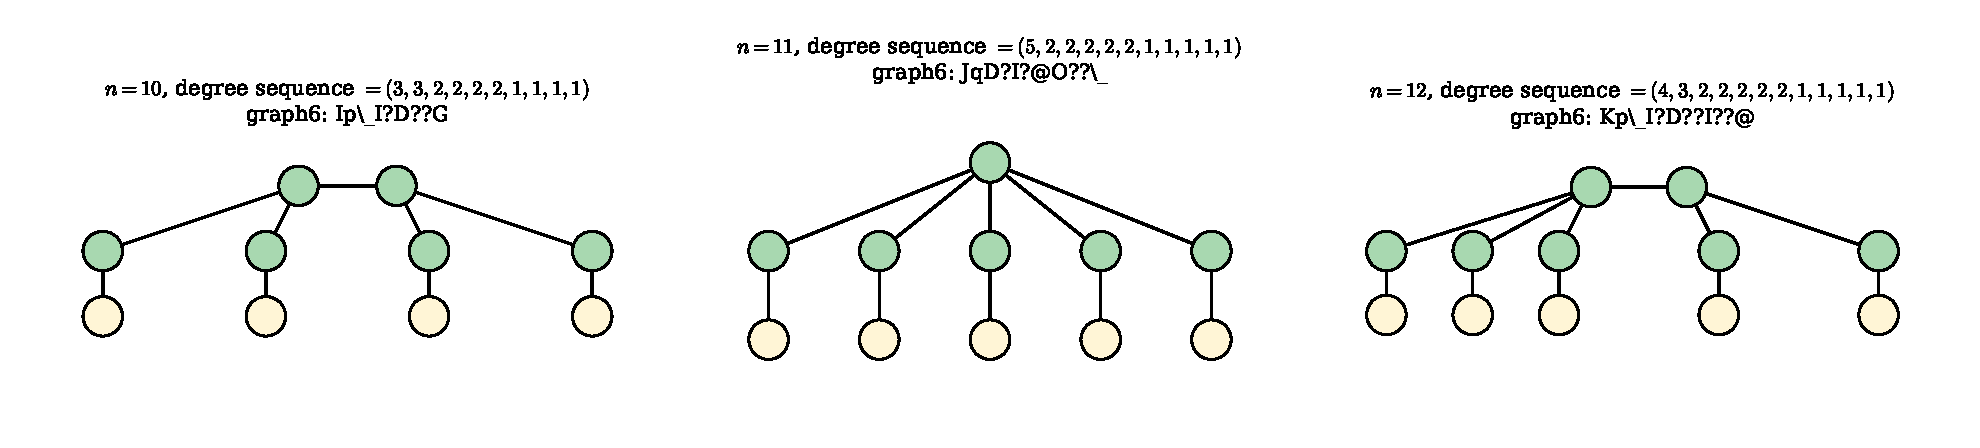
\includegraphics[width=\linewidth]{fig10_caterpillar_maximizers.pdf}
\caption{Maximizers of $W(T; -1, -1, 1)$ over all non-isomorphic trees of order $n$, for $n = 10, 11, 12$. Internal vertices are coloured green and leaves cream. None of the three trees is a caterpillar (the non-leaf vertices do not form a path). $n = 11$ is the spider $S^{(2)}_{5}$ with $h = (11 - 1)/2 = 5$ length-$2$ spokes; $n = 10$ is the balanced double-spider $DS(3, 3)$; and $n = 12$ is $DS(4, 3)$.}
\label{fig:caterpillar_maximizers}
\end{figure}

The pattern in Table~\ref{tab:caterpillar_argmax} and
Figure~\ref{fig:caterpillar_maximizers} is the central empirical
phenomenon of the paper: a parameter triple at which the
classical star/path extremals fail and the observed maximizer is
not even a caterpillar for $7 \le n \le 20$, with a sharp
odd/even structural pattern. The corresponding formal conjecture
is stated in Section~\ref{sec:conclusion}.

% =====================================================================
\section{Sensitivity analysis}\label{sec:sensitivity}
% =====================================================================

The Wuzi family is benchmarked on three established chemical
compound classes used as testbeds for parametric topological
indices in the literature: the $18$ octane isomers, the $106$
non-isomorphic trees of order $10$, and the $75$ decane isomers.
The benchmark protocol follows the conventions of
Sections~5.1, 5.3, and 5.4
of~\cite{MovahediGutmanRedzepovicFurtula2026}.

\subsection{Property correlations on the octane isomers}\label{sec:octanes}

Table~\ref{tab:octane_competitor} reports the Pearson correlation
$r$ between each index and each of the five physicochemical
properties of the $n = 18$ octane isomers (boiling point $T_B$,
enthalpy of formation $\Delta H_f$, enthalpy of vaporization
$\Delta H_{\mathrm{vap}}$, entropy $S$, acentric factor $\omega$;
property data from the NIST WebBook), with the Wuzi family
sampled at eight canonical parameter triples and compared
head-to-head against eight classical bond-incident-degree indices
($M_1, M_2, R, SO, GA, H, ABC, AZI$) computed on the same
$18$-row octane table.

\begin{table}[H]
\centering
\caption{Pearson correlation $r$ between each index and each of the five physicochemical properties of the $18$ octane isomers. Sign carries the index's natural direction; what matters chemically is $|r|$. Bold entries flag the per-column maximum $|r|$ across all listed indices. Bootstrap uncertainty (B = 10\,000, percentile method, 95\% CI): headline values are $r(\Delta H_{\mathrm{vap}}, GA) = +0.959$ with CI $[+0.917, +0.986]$, $r(\Delta H_{\mathrm{vap}}, H) = +0.959$ with CI $[+0.917, +0.986]$, and $r(\Delta H_{\mathrm{vap}}, W(0,0,2)) = -0.967$ with CI $[-0.991, -0.921]$. The CI half-widths range from $0.019$ to $0.47$, median $0.13$; differences in $|r|$ smaller than ${\sim}0.10$--$0.15$ are within bootstrap noise at $n = 18$. A leave-one-out cross-validation across the $18$ isomers gives maximum drift in $|r|$ of at most $0.011$ on the headline $\Delta H_{\mathrm{vap}}$ cells, attributable to $2,3,3$-trimethylpentane, confirming that the headline correlations are not driven by a single outlying isomer.}
\label{tab:octane_competitor}
\small
\begin{tabular}{llrrrrr}
\toprule
Index & Family & $r(T_B)$ & $r(\Delta H_f)$ & $r(\Delta H_{\mathrm{vap}})$ & $r(S)$ & $r(\omega)$\\
\midrule
$M_1$              & classical & $-0.718$ & $-0.762$ & $-0.912$ & $-0.973$ & $-0.970$\\
$M_2$              & classical & $-0.503$ & $-0.553$ & $-0.775$ & $-0.942$ & $-0.987$\\
$R$                & classical & $+0.821$ & $+0.848$ & $+0.956$ & $+0.935$ & $+0.901$\\
$SO$               & classical & $-0.748$ & $-0.793$ & $-0.926$ & $-0.969$ & $-0.957$\\
$GA$               & classical & $+0.823$ & $+0.856$ & $+0.959$ & $+0.942$ & $+0.909$\\
$H$                & classical & $+0.822$ & $+0.846$ & $+0.959$ & $+0.935$ & $+0.904$\\
$ABC$              & classical & $-0.869$ & $-0.892$ & $-0.944$ & $-0.858$ & $-0.790$\\
$AZI$              & classical & $\mathbf{+0.936}$ & $\mathbf{+0.922}$ & $+0.929$ & $+0.734$ & $+0.656$\\
\midrule
$W(1, 0, 0)$       & Wuzi      & $-0.503$ & $-0.553$ & $-0.775$ & $-0.942$ & $\mathbf{-0.987}$\\
$W(-1/2, 0, 0)$    & Wuzi      & $+0.821$ & $+0.848$ & $+0.956$ & $+0.935$ & $+0.901$\\
$W(0, -1/2, 0)$    & Wuzi      & $+0.801$ & $+0.829$ & $+0.953$ & $+0.950$ & $+0.927$\\
$W(0, -1, 0)$      & Wuzi      & $+0.822$ & $+0.846$ & $+0.959$ & $+0.935$ & $+0.904$\\
$W(0, 0, 1)$       & Wuzi      & $-0.828$ & $-0.831$ & $-0.966$ & $-0.931$ & $-0.930$\\
$W(0, 0, 2)$       & Wuzi      & $-0.830$ & $-0.844$ & $\mathbf{-0.967}$ & $-0.939$ & $-0.926$\\
$W(1, 1, 1)$       & Wuzi      & $-0.615$ & $-0.677$ & $-0.840$ & $-0.959$ & $-0.981$\\
$W(-1, -1, 1)$     & Wuzi      & $+0.763$ & $+0.830$ & $+0.747$ & $+0.632$ & $+0.494$\\
\bottomrule
\end{tabular}
\end{table}

Three structural observations follow from
Table~\ref{tab:octane_competitor}.

\begin{enumerate}[label=(\alph*)]
\item At the four exact-reduction parameter triples
($(1, 0, 0), (-1/2, 0, 0), (0, -1/2, 0), (0, -1, 0)$) the Wuzi
correlations coincide with those of the corresponding classical
indices $M_2, R, \chi, H/2$ to within floating-point precision,
in agreement with Proposition~\ref{prop:reductions}; these rows
function as an internal consistency check.

\item The strongest absolute correlation on $T_B$ and on
$\Delta H_f$ is attained by the augmented Zagreb index $AZI$
($|r| = 0.936$ and $|r| = 0.922$ respectively); no Wuzi
parameter triple in the sampled panel exceeds it. On
$\Delta H_{\mathrm{vap}}$ the strongest correlation is the
pure-$\gamma$ triple $W(0, 0, 2)$ with $|r| = 0.967$, and the
runners-up $GA$ and $H$ both attain $|r| = 0.959$. The $0.008$
margin between $W(0, 0, 2)$ and $GA / H$ is well within the
bootstrap-CI half-width of approximately $0.034$ at $n = 18$
(see the table caption), so the three indices are statistically
indistinguishable on this benchmark and no claim of superiority
is made. On the acentric factor $\omega$ the strongest is
$W(1, 0, 0) = M_2$ with $|r| = 0.987$, which is by
Proposition~\ref{prop:reductions} the second Zagreb index itself.

\item A leave-one-out cross-validation across the $18$ isomers
confirms that the headline correlations are not driven by single
outlying octanes: the maximum drift in $|r|$ across the $18$
leave-one-outs is at most $0.011$ on the headline
$\Delta H_{\mathrm{vap}}$ cells ($0.008$ for $GA$, $0.008$ for
$H$, and $0.011$ for $W(0, 0, 2)$), with the largest drift in
each case attributable to the same isomer
($2, 3, 3$-trimethylpentane).
\end{enumerate}

Table~\ref{tab:octane_competitor} is a univariate
sensitivity benchmark, not a multivariate QSPR validation: a
single scalar index correlating strongly with one property on
$18$ isomers can still be multivariately redundant with the
classical baseline. The multivariate redundancy question is the
subject of the companion methodology
paper~\cite{Paper2_Screening}, which evaluates the Wuzi family
on three larger MoleculeNet datasets.

\begin{remark}
The edge-Padmakar--Ivan index $PI$ is degenerate on the $18$
octanes ($\sigma = 0$, mean $42$) and is therefore excluded from
the comparison. The degeneracy is structural: for every tree $T$
of size $m$, removing any edge $e$ disconnects $T$ into two
components, and because trees have unique shortest paths every
other edge lies entirely in one component or the other (no
equidistant edges arise on a tree). Hence the edge-$PI$
contribution from $e$ is $m - 1$, and summing over the $m$ edges
gives $PI(T) = m(m - 1)$. The $18$ octanes are all trees on $8$
vertices, giving $PI \equiv 7 \cdot 6 = 42$.
\end{remark}

Figure~\ref{fig:octanes} shows the full signed-$r$ heatmap on the
five-property octane table for the $30$-index classical baseline
together with selected Wuzi parameter triples.

\begin{figure}[H]
\centering
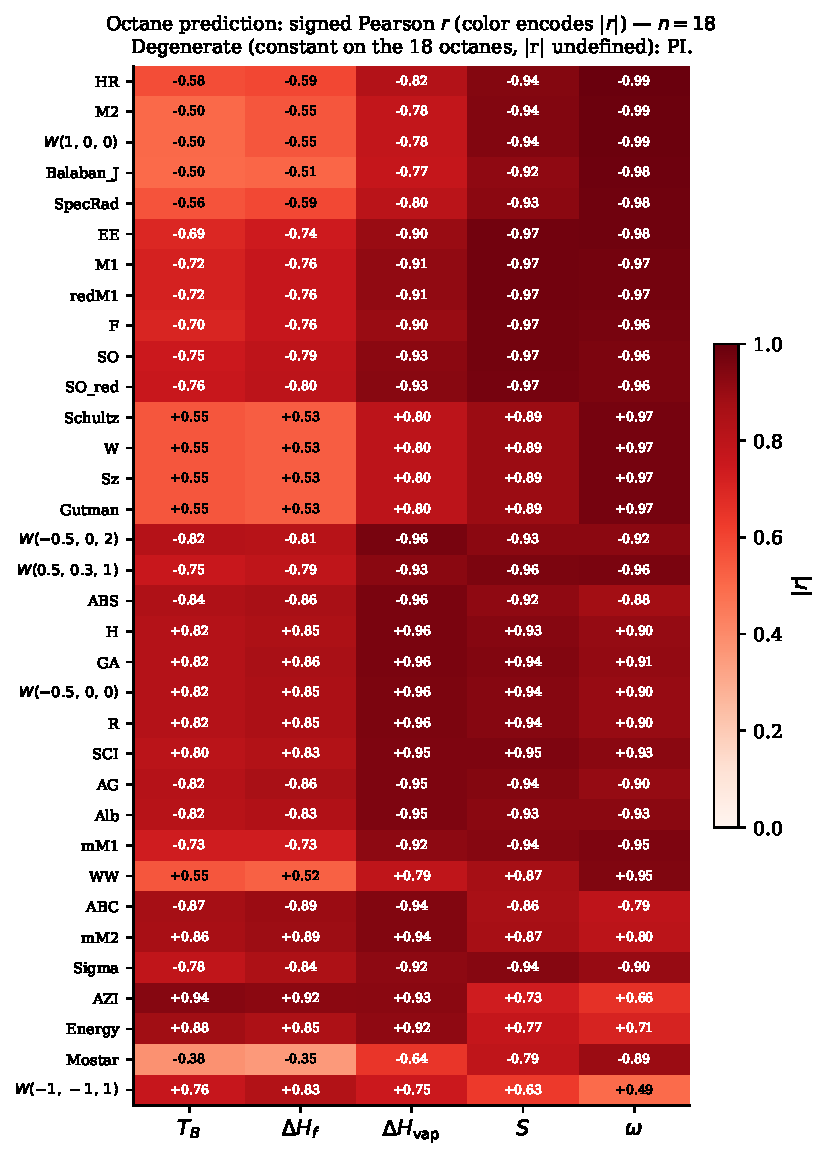
\includegraphics[width=0.95\linewidth]{fig4_octane_heatmap.pdf}
\caption{Signed Pearson $r$ between each Wuzi/classical index and each of the five octane physicochemical properties ($T_B$, $\Delta H_f$, $\Delta H_{\mathrm{vap}}$, $S$, $\omega$) on the $18$ isomers. Color encodes $|r|$; values are printed with sign. $PI$ is degenerate on the dataset and removed.}
\label{fig:octanes}
\end{figure}

\subsection{Degeneracy on trees of order 10}\label{sec:degeneracy}

Following the protocol of
\cite{MovahediGutmanRedzepovicFurtula2026} Section~5.3,
Figure~\ref{fig:degeneracy} reports the degeneracy of each index
on the $106$ non-isomorphic trees of order $10$, where degeneracy
is the fraction of pairs of distinct trees on which the index
takes the same value. The Wuzi family at $\gamma = 2$ attains
degeneracy of approximately $25\%$, comparable to the
Sombor-family range of $17$--$22\%$ reported in
\cite{MovahediGutmanRedzepovicFurtula2026} Figure~5.

\begin{figure}[H]
\centering
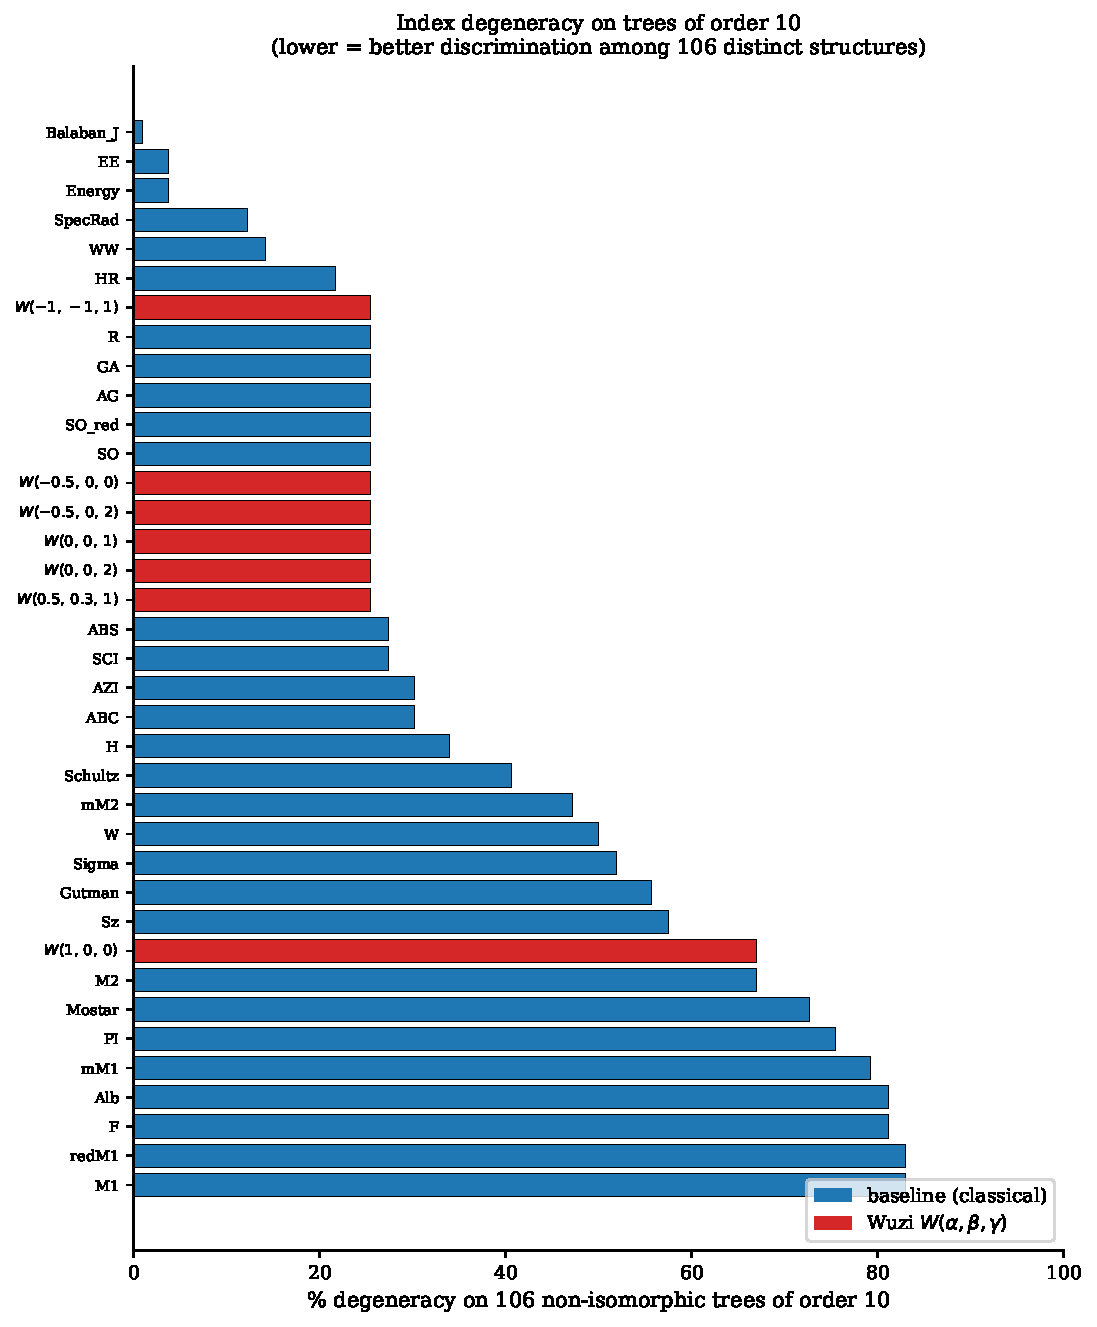
\includegraphics[width=0.85\linewidth]{fig6_degeneracy_bars.pdf}
\caption{Percent degeneracy on $106$ non-isomorphic trees of order $10$ for each of the $30$ baseline indices and selected Wuzi parameter points.}
\label{fig:degeneracy}
\end{figure}

\subsection{Structure sensitivity on decane isomers}\label{sec:ss}

Following the protocol of
\cite{MovahediGutmanRedzepovicFurtula2026} Section~5.4,
Figure~\ref{fig:ss} reports the structure-sensitivity metrics
$SS = \sigma/\mu$, $Abr = (\max - \min)/\mu$, and $SA = SS/Abr$
for the top $20$ indices by $SS$ on the $75$ decane isomers. The
Wuzi family values lie in the same regime as the Sombor variants
reported in \cite{MovahediGutmanRedzepovicFurtula2026} Table~2.

\begin{figure}[H]
\centering
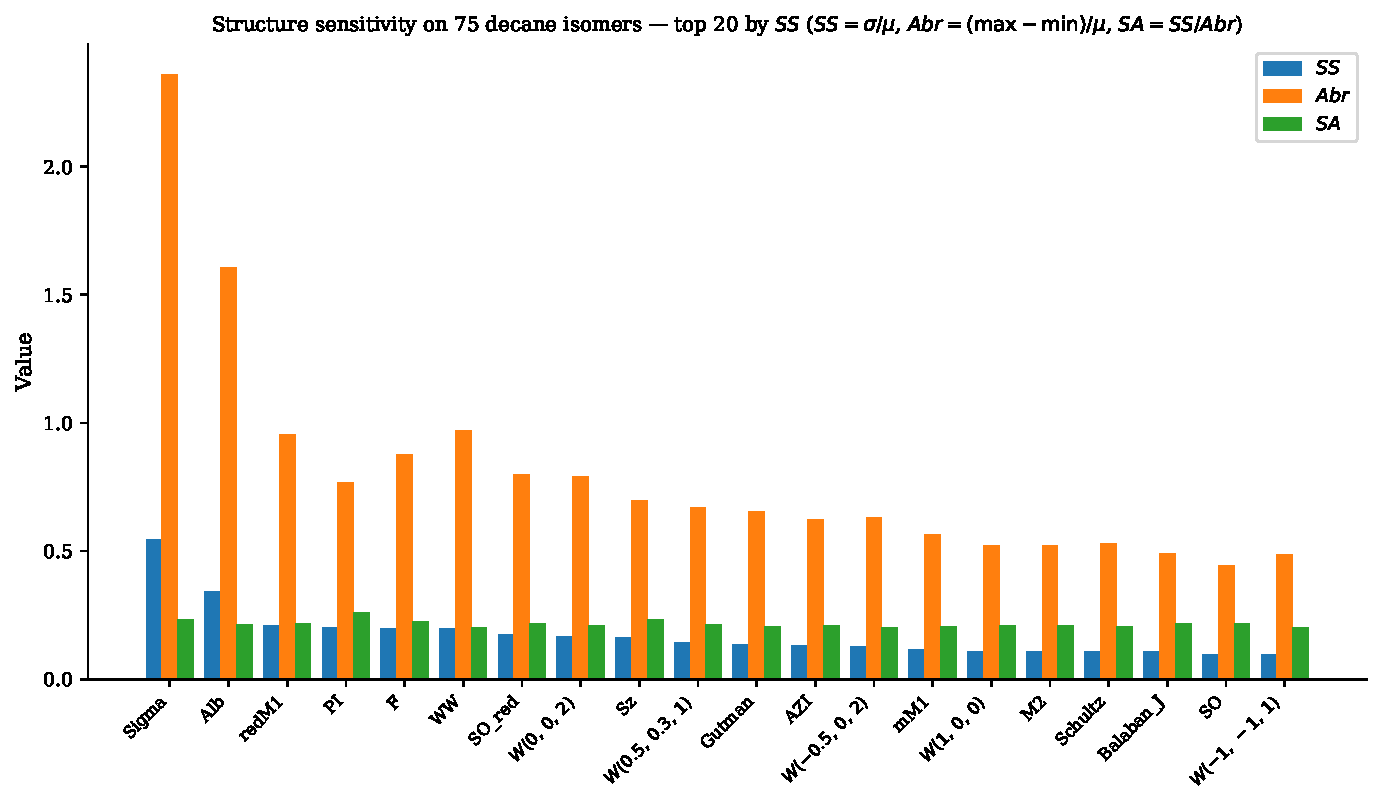
\includegraphics[width=0.95\linewidth]{fig7_structure_sensitivity.pdf}
\caption{Structure-sensitivity metrics on the $75$ decane isomers, top $20$ indices by $SS$.}
\label{fig:ss}
\end{figure}

% =====================================================================
\section{Concluding remarks and open problems}\label{sec:conclusion}
% =====================================================================

The Wuzi family combines mathematical tractability on the
standard graph classes with an explicit structural ceiling on its
chemometric reach. The rigorous core of Section~\ref{sec:bounds}
gives a coherent set of bounds: the bracket bound via the
edge-contribution function (Proposition~\ref{thm:bracket}) and the
uniform ratio bound (Theorem~\ref{thm:ratio_bound}) together
sandwich $\Wuzi$ in terms of any classical BID index with strictly
positive edge contribution, and the Jensen-type and
Cauchy--Schwarz inequalities of \S\ref{sub:cs}--\S\ref{sub:R_chi_SO}
close the picture in $M_1, M_2, R, \chi$, and $SO$ for the
non-negative parameter region. The structural observation
recorded in Section~\ref{sec:intro} (every BID index on
$\mathcal{G}_4$ lies in a vector space of dimension at most ten)
gives the reason that no parametric BID family on $\mathcal{G}_4$
--- including the Wuzi family --- can escape the ten-dimensional
BID subspace; the companion methodology
paper~\cite{Paper2_Screening} exploits this fact for cross-dataset
redundancy screening.

The empirical centrepiece is the non-classical extremal regime at
$(\alpha, \beta, \gamma) = (-1, -1, 1)$: exhaustive enumeration of
all non-isomorphic trees up to order $n = 20$ shows that the
maximizer is neither the star, the path, nor a caterpillar for
$n \ge 7$ (Table~\ref{tab:caterpillar_argmax}). Let
$S^{(2)}_{h}$ denote the spider with hub degree $h$ and length-$2$
spokes (the tree on $2h + 1$ vertices consisting of a single hub
of degree $h$ together with $h$ length-$2$ paths), and let
$DS(a, b)$ denote the balanced double-spider with hub degrees
$a, b$ (the tree on $2(a + b - 1)$ vertices obtained by joining
two hubs of degrees $a$ and $b$ by an edge and attaching $a - 1$
and $b - 1$ length-$2$ paths to the respective hubs). The
exhaustive enumeration supports the following conjecture.

\begin{conjecture}[Mixed-sign extremal trees: spider/double-spider]\label{conj:caterpillar_max}
For the parameter triple $(\alpha, \beta, \gamma) = (-1, -1, 1)$
and tree order $n \ge 9$,
\begin{enumerate}[label=(\alph*)]
\item if $n$ is odd, the unique maximizer of $W(T; -1, -1, 1)$
over all non-isomorphic trees $T$ of order $n$ is the spider
$S^{(2)}_{(n - 1)/2}$;
\item if $n$ is even, the unique maximizer is the balanced
double-spider $DS(a, b)$ with $a + b = n/2 + 1$ and
$|a - b| \le 1$.
\end{enumerate}
In both cases the maximizer is non-caterpillar.
\end{conjecture}

The conjecture is supported by exhaustive enumeration through
$n = 20$. The natural proof template is the classical
transformation-lemma approach: show that any tree $T$ of order
$n$ not isomorphic to the prediction admits a local edge
transformation that strictly increases $W(T; -1, -1, 1)$. This
formal proof is left as the main mathematical open problem of the
paper.

A further set of open problems --- sharp Nordhaus--Gaddum sum
bounds for $\Wuzi$ in the spirit of the classical Zagreb-index
results~\cite{NordhausGaddumOrig1956}; sharp two-sided bounds via
the geometric--arithmetic index
$GA$~\cite{VukicevicFurtula2009GA}, the harmonic index $H$, and
the atom-bond-connectivity index $ABC$; and formal extremal-graph
characterisations for unicyclic and bicyclic graphs in the
spirit of~\cite{LiuLuTian2008Randic}
and~\cite{HansenMelot2003unicyclicRandic} --- are natural
extensions of the bounds programme of Section~\ref{sec:bounds}.
On the chemometric side, the natural extensions are to additional
compound classes (benzene derivatives, alkane homologues beyond
octane and decane) and to compound-class-specific QSPR endpoints,
together with a formal study of the
Albertson~\cite{Albertson1997} irregularity pairing
$\mathrm{Alb}(G) = \sum_{uv \in E(G)} |d_u - d_v|$ that is the
natural mathematical companion of the Wuzi $\gamma$-axis.

The Wuzi family is therefore best viewed not as a claim of
universal QSPR superiority --- the family is explicitly shown to
sit inside the same finite-dimensional BID descriptor subspace as
the established classical indices, and its octane correlations
are in the same regime as theirs --- but as a controlled
parametric probe of that finite BID descriptor space, with the
mixed-sign spider/double-spider regime at
$(\alpha, \beta, \gamma) = (-1, -1, 1)$ providing the paper's
main new extremal phenomenon.

\acknowledgment{The authors thank colleagues for discussions of
the computational extremal-graph search and the
redundancy-screening protocol. Funding sources and institutional
support to be acknowledged in the final version of the
manuscript.}

% References should be ordered alphabetically.
% We noticed that in recent papers, there are some nonexistent references.
% It is forbidden to do such unethical things. Manuscripts that contain
% non-existent references will be immediately rejected, and their corresponding
% authors will be black-listed.
\singlespacing
\begin{thebibliography}{99}

\bibitem{Albertson1997} M. O. Albertson, The irregularity of a
    graph, \textit{Ars Combin.\/} \textbf{46} (1997) 219--225.

\bibitem{BarmanDas2026HSO} J. Barman, S. Das, Geometric approach
    to degree-based topological index: Hyperbolic Sombor index,
    \textit{MATCH Commun. Math. Comput. Chem.\/}
    \textbf{95} (2026) 63--94.

\bibitem{BollobasErdos1998} B. Bollob\'as, P. Erd\H{o}s,
    Graphs of extremal weights,
    \textit{Ars Combin.\/} \textbf{50} (1998) 225--233.

\bibitem{BorovicaninDasFurtulaGutman2017Zagreb} B. Borovi\'canin,
    K. C. Das, B. Furtula, I. Gutman, Bounds for Zagreb indices,
    \textit{MATCH Commun. Math. Comput. Chem.\/}
    \textbf{78} (2017) 17--100.

\bibitem{DasCevikCangulShang2021Sombor} K. C. Das, A. S. \c{C}evik,
    I. N. Cangul, Y. Shang, On Sombor index,
    \textit{Symmetry\/} \textbf{13} (2021) \#140.

\bibitem{DasGutman2022SomborTrees} K. C. Das, I. Gutman,
    On Sombor index of trees,
    \textit{Appl. Math. Comput.\/}
    \textbf{412} (2022) \#126575.

\bibitem{Fajtlowicz1987Harmonic} S. Fajtlowicz, On conjectures of
    Graffiti-II, \textit{Congr. Numer.\/} \textbf{60} (1987) 187--197.

\bibitem{FurtulaGutman2015F} B. Furtula, I. Gutman, A forgotten
    topological index, \textit{J. Math. Chem.\/}
    \textbf{53} (2015) 1184--1190.

\bibitem{Gutman1972} I. Gutman, N. Trinajsti\'c, Graph theory and
    molecular orbitals. Total $\pi$-electron energy of alternant
    hydrocarbons, \textit{Chem. Phys. Lett.\/}
    \textbf{17} (1972) 535--538.

\bibitem{GutmanFurtula2008Randic} I. Gutman, B. Furtula (Eds.),
    \textit{Recent Results in the Theory of Randi\'c Index\/},
    Mathematical Chemistry Monographs MCM-6, University of
    Kragujevac and Faculty of Science Kragujevac, Kragujevac, 2008.

\bibitem{GutmanToganYurttasCevikCangul2018Sigma} I. Gutman,
    M. Togan, A. Yurtta\c{s}, A. S. \c{C}evik, I. N. Cangul,
    Inverse problem for sigma index,
    \textit{MATCH Commun. Math. Comput. Chem.\/}
    \textbf{79} (2018) 491--508.

\bibitem{Gutman2021SomborBasic} I. Gutman, Some basic properties
    of Sombor indices,
    \textit{Open J. Discr. Appl. Math.\/}
    \textbf{4} (2021) 1--3.

\bibitem{Gutman2021Sombor} I. Gutman, Geometric approach to
    degree-based topological indices: Sombor indices,
    \textit{MATCH Commun. Math. Comput. Chem.\/}
    \textbf{86} (2021) 11--16.

\bibitem{GutmanFurtulaOz2024Elliptic} I. Gutman, B. Furtula,
    M. S. Oz, Geometric approach to vertex-degree-based topological
    indices: Elliptic Sombor index, theory and application,
    \textit{Int. J. Quantum Chem.\/}
    \textbf{124} (2024) \#e27346.

\bibitem{HansenMelot2003unicyclicRandic} P. Hansen, H. M\'elot,
    Variable neighborhood search for extremal graphs. 6.
    Analysing bounds for the connectivity index,
    \textit{J. Chem. Inf. Comput. Sci.\/}
    \textbf{43} (2003) 1--14.

\bibitem{LiuLuTian2008Randic} H. Liu, M. Lu, F. Tian, On the
    Randi\'c index, \textit{J. Math. Chem.\/}
    \textbf{44} (2008) 301--310.

\bibitem{MendezBermudezAguilarSanchez2022MeanSombor}
    J. A. M\'endez-Berm\'udez, R. Aguilar-S\'anchez,
    E. D. Molina, J. M. Rodr\'iguez, Mean Sombor index,
    \textit{Discr. Math. Lett.\/}
    \textbf{9} (2022) 18--25.

\bibitem{MilovanovicMilovanovicMatejic2021Sombor} I. Milovanovi\'c,
    E. Milovanovi\'c, M. Mateji\'c, On some mathematical properties
    of Sombor indices,
    \textit{Bull. Int. Math. Virtual Inst.\/}
    \textbf{11} (2021) 341--353.

\bibitem{Movahedi2025DSO} F. Movahedi, Diminished Sombor index and
    its relationship with topological indices,
    \textit{Filomat\/} \textbf{39} (2025) 10519--10532.

\bibitem{MovahediGutmanRedzepovicFurtula2026} F. Movahedi,
    I. Gutman, I. Red\v{z}epovi\'c, B. Furtula,
    Diminished Sombor index,
    \textit{MATCH Commun. Math. Comput. Chem.\/}
    \textbf{95} (2026) 141--162.

\bibitem{NikolicKovacevicMilicevicTrinajstic2003} S. Nikoli\'c,
    G. Kova\v{c}evi\'c, A. Mili\v{c}evi\'c, N. Trinajsti\'c,
    The Zagreb indices 30 years after,
    \textit{Croat. Chem. Acta\/} \textbf{76} (2003) 113--124.

\bibitem{NordhausGaddumOrig1956} E. A. Nordhaus, J. W. Gaddum,
    On complementary graphs, \textit{Amer. Math. Monthly\/}
    \textbf{63} (1956) 175--177.

\bibitem{Randic1975} M. Randi\'c, On characterization of
    molecular branching, \textit{J. Am. Chem. Soc.\/}
    \textbf{97} (1975) 6609--6615.

\bibitem{Paper2_Screening} G. Shiwakoti, A. Natarajan,
    M. Arockiaraj, Orthogonality screening of topological
    indices for QSPR modeling: a structural and empirical
    redundancy analysis, in preparation, 2026.

\bibitem{VukicevicFurtula2009GA} D. Vuki\v{c}evi\'c, B. Furtula,
    Topological index based on the ratios of geometrical and
    arithmetical means of end-vertex degrees of edges,
    \textit{J. Math. Chem.\/} \textbf{46} (2009) 1369--1376.

\bibitem{Vukicevic2010BondAdditive2} D. Vuki\v{c}evi\'c, Bond
    additive modeling 2. Mathematical properties of max-min
    rodeg index,
    \textit{Croat. Chem. Acta\/}
    \textbf{83} (2010) 261--273.

\bibitem{WagnerWang2018ChemGraphTheory} S. Wagner, H. Wang,
    \textit{Introduction to Chemical Graph Theory\/},
    Chapman \& Hall/CRC, Boca Raton, 2018.

\bibitem{WangMaoLiFurtula2022SomborRelations} Z. Wang, Y. Mao,
    Y. Li, B. Furtula, On relations between Sombor and other
    degree-based indices,
    \textit{J. Appl. Math. Comput.\/}
    \textbf{68} (2022) 1--17.

\bibitem{Wiener1947} H. Wiener, Structural determination of
    paraffin boiling points, \textit{J. Am. Chem. Soc.\/}
    \textbf{69} (1947) 17--20.

\bibitem{ZhouTrinajstic2009sumconn} B. Zhou, N. Trinajsti\'c,
    On a novel connectivity index, \textit{J. Math. Chem.\/}
    \textbf{46} (2009) 1252--1270.

\end{thebibliography}

\end{document}
